\newcommand{\subparagraph}{}  

\documentclass[journal]{IEEEtran}
\usepackage{graphicx}
\usepackage{amsmath}
\usepackage{titlesec}
\usepackage{listings}
\usepackage{color} 
\usepackage{subcaption}

\DeclareMathOperator{\sech}{sech}


\pagestyle{empty}


\begin{document}
	
\title{Investigation of Dust-Ion Acoustic Solitary Structures in a Weakly Relativistic Plasma}
\author{S. Ramesh, C. Verma, and S. Chandra}

\thanks{Shashank Ramesh is with Physics Department, Kirori Mal College, University of Delhi, India (email - shashankramesh38@hotmail.com)}
\thanks{Chirag Verma is with Physics Department, Kirori Mal College, University of Delhi, India. (email - chirag2000verma@gmail.com)}
\thanks{Swarniv Chandra was the program coordinator for the Summer Workshop on Plasma Physics 2020 (e-mail: swarniv147@gmail.com).}
\maketitle
\thispagestyle{empty}

\begin{abstract}
In this paper, analytical investigation of dust-ion acoustic waves
in a weak relativistically degenerate plasma, with mobile negatively charged dust particles and usual ions and electron components is carried out. The Kortweg-de Vries equation is also derived, to study solitary waves, using relevant stretched coordinates and perturbation expansion.
\end{abstract}

\renewcommand\IEEEkeywordsname{PACS}
	
\begin{IEEEkeywords}
	52.27.Lw; 52.27.Ny; 52.25.Ya.
\end{IEEEkeywords}


\renewcommand\IEEEkeywordsname{Keywords}

\begin{IEEEkeywords}
	Dust ion acoustic wave; KdV equation; solitary structures.
\end{IEEEkeywords}

\renewcommand\IEEEkeywordsname{Nomenclature}

\begin{IEEEkeywords}
KdV: Korteweg-de Vries
\end{IEEEkeywords}

\IEEEpeerreviewmaketitle


\section{Introduction}

	\IEEEPARstart{D}{ust} ion acoustic waves are an expanding area of research, and with the recognition of quantum and relativistic effects involved in these phenomena, more opportunities come up for investigation of these waves in various regimes. A number of analytical treatments have been carried out already regarding these waves over the past years. More importantly, dust plasmas have been observed in active galactic nuclei \cite{1}, laser fields \cite{2}, pulsar magnetospheres [3] and polar regions of neutron stars [4], making it a huge region of interest for astrophysics. There is also evidence for presence of these dustplasmas in the early stages of the Universe [5], [6], [7] and the centre of the milky way galaxy [8] Occurrences of relativistic plasma were found in Van Allen radiation belt [9] and the boundary layer of earth’s magnetosphere too [10]. This has led to extensive research concerning these waves. Different types of dust acoustic waves have been studied by Mamun and Shukla (2002) [11], Rao et al (1990) [12] and others. Rao et al characterized the linear normal modes and nonlinear supersonic solitons and Mamunand Shukla characterized spherical and cylindrical waves as opposed to one dimensional waves. These waves have also been studied with various pseudopotential approaches, such as in Pakzad (2009) [13]. Magnetized plasmas have also been found to have rarefactive solitons in Kundu et al (2013) [14] where soliton width decreases with magnitude of the field. HF Liu et al (2010) [15] have used a modified KdV-Burgers equation to model cylindrical and spherical dust ion acoustic waves in weakly relativistic plasma. Solitary structures are observed in these models that vary with density of the components, the mass of the constituent particles and temperatures of the components. Chetia [16] studied compressive and rarefactive Ion-Acoustic solitons. Also, Chandra, Paul, and Ghosh [17] have showed that relativistic degeneracy parameter significantly influences the conditions of formation and properties of solitary structures. In this paper, we have considered the model consisting of mobile negatively charged dust particles, singly charged ions and electrons to derive the linear dispersion relation and Korteweg-de Vries equations in weakly relativistic regime using standard perturbation techniques. The effects of varying temperatures, dust charge and other parameters are studied. We have divided the paper in five sections (more or less). The second section throws some light on the basic quantum hydrodynamic, and three fluid equations; along with a relativistically degenerate pressure scheme. The next section focusses on the derivation of linear dispersion relation. We have also derived the KdV equation, and its solution for the same set of equations in the third section. We discuss some graphical properties of the above derived equations in the fourth section.

\section{Basic Formulation}

	\normalsize In order to analytically study the propagation of solitary waves in an unmagnetized three component weak relativistically degenrate plasma we start with a set of interpenetrating fluids (three, here) characterized by :
	
	\begin{enumerate}
		\item The equations of continuity and motion of 
		\begin{itemize}
			\item ions,
			\item electrons, and
			\item dust particles
		\end{itemize}
		\item The Poisson's equation
		\item The Pressure Law
	\end{enumerate}

\subsection{Governing Equations }

\begin{itemize}
		\item{For Dust particles}:
		\\*
		\begin{equation}
				\frac{\partial n_d}{\partial t} + \frac{\partial (n_du_d)}{\partial x} = 0	
		\end{equation}
		\begin{equation}
			\frac{\partial u_d}{\partial t} + u_d \frac{\partial u_d}{\partial x} = \frac{Q_d}{m_d}\frac{\partial \phi}{\partial x}
		\end{equation}		
		
		\item {For Ions}:
		\begin{equation}
			\frac{\partial n_i}{\partial t} + \frac{\partial (n_iu_i)}{\partial x} = 0		
		\end{equation}
		
		\begin{equation}
			\frac{\partial u_i}{\partial t} + u_i \frac{\partial u_i}{\partial x} = -\frac{Q_i}{m_i} \frac{\partial \phi}{\partial x} - \frac{1}{m_in_i} \frac{\partial p_i}{\partial x}
		\end{equation}		
		
		\item {For Electrons}:
		\begin{equation}
			\frac{\partial n_e}{\partial t} + \frac{\partial (n_eu_e)}{\partial x} = 0
		\end{equation}
		
		
		\begin{equation}
		\begin{split}
			\frac{\partial u_e}{\partial t} + u_e \frac{\partial u_e}{\partial x} = -\frac{Q_e}{m_e} \frac{\partial \phi}{\partial x} - \frac{1}{m_en_e} \frac{\partial p_e}{\partial x} &\\
			+ \frac{\hbar^2}{2m_e^2} \frac{\partial}{\partial x} (\frac{1}{\sqrt{n_e}}\frac{\partial^2 \sqrt{n_e}}{\partial x^2})&
		\end{split}
		\end{equation}
		
		\item {Poisson's Equation:}
		
		\begin{equation}
			\frac{\partial^2 \phi}{\partial x^2} = 4\pi(Q_en_e - Q_in_i + Q_dn_d)
		\end{equation}	
		
	\end{itemize}


\subsection{Pressure Law}
	Following from Chandrasekhar (1939), The electron degeneracy pressure in fully degenerate and relativistic form can be expressed as : 

		\begin{equation}
				p_j = (\pi m_e^4c^5/3h^3)[R_j(2R_j^2 - 3)\sqrt{1 + R_j^2} + 3 \sinh^{-1}R_j] 
		\end{equation}
		
		\begin{equation}
			R_j = {p_F}_j/m_ec = [3h^3n_j/8\pi m_e^3c^3]^{1/3}= R_{j0}n_j^{1/3}
		\end{equation}
		
		\begin{equation*} 
			{R_j}_0 = (n_{j0}/n_0)^{1/3} = 5.9 \cdot 10^{29} cm^{-1}
		\end{equation*}
		
		For weak-relativistic degeneracy : $R_j\rightarrow 0$, and, hence
		
		\begin{equation*}
			p_j = \frac{1}{20}(\frac{3}{\pi})^{\frac{2}{3}}\frac{h^2}{m_e}n_j^{\frac{5}{3}}
		\end{equation*}

		where the suffices $d, e, i$ stand for dust particle, electron, and ion components respectively; $u_j$ and $p_j$ are respectively the fluid velocity and degeneracy pressure of the $j^{th}$ species, i.e. electron or dust particle or ion; $\phi$ is the electrostatic wave potential; and $Q_j$ is the charge on the $j^{th}$ species.

	\subsection{Normalized Equations}

			Under the following normalized scheme:
			$n_j \rightarrow n_j/{n_i}_0, t \rightarrow t\omega_{pd}, x \rightarrow x/\lambda_{De}, u_j \rightarrow u_j/C_d, \phi \rightarrow K_bT_e/m_d$ \\*\\*
			where $\omega_{pd} = (m_d/4\pi {n_i}_0 e^2)^{1/2}$ is the characteristic dust plasma frequency, $\lambda_{De} = (K_bT_e/4\pi {n_i}_0 e^2)^{1/2}$ is the Debye length, $C_d = (K_bT_e/m_d)^{1/2}$ is the dust acoustic speed; the above equations are then normalized to:
	
			\begin{equation}
				\frac{\partial n_d}{\partial t} + \frac{\partial (n_du_d)}{\partial x} = 0	
			\end{equation}
		
			\begin{equation}
				\frac{\partial u_d}{\partial t} + u_d \frac{\partial u_d}{\partial x} = -Z_d\frac{\partial \phi}{\partial x}
			\end{equation}			 
	
			\begin{equation}
				\frac{\partial n_i}{\partial t} + \frac{\partial (n_iu_i)}{\partial x} = 0		
			\end{equation}
		
			\begin{equation}
				\frac{\partial u_i}{\partial t} + u_i \frac{\partial 	u_i}{\partial x} = -\frac{1}{Q}( \frac{\partial \phi}{\partial x} + \frac{\alpha}{n_i} \frac{\partial p_i}{\partial x})
			\end{equation}

			\begin{equation}
				\frac{\partial n_e}{\partial t} + \frac{\partial (n_eu_e)}{\partial x} = 0
			\end{equation}
		
			\begin{equation}
				\begin{split}
					\frac{\partial u_e}{\partial t} + u_e \frac{\partial u_e}{\partial x} = -\frac{1}{P}(\frac{\partial \phi}{\partial x} + \frac{1}{n_e} \frac{\partial p_e}{\partial x})  + \frac{1}{P^2}\frac{H^2}{2} \frac{\partial}{\partial x} (\frac{1}				{\sqrt{n_e}}\frac{\partial^2 \sqrt{n_e}}{\partial x^2})
				\end{split}
			\end{equation}
	
			\begin{equation}
				\frac{\partial^2 \phi}{\partial x^2} = (n_e - n_i + Z_dn_d)
			\end{equation}
		
			where $Q = \frac{m_i}{m_d}, P = \frac{m_e}{m_d}, H = \frac{\hbar w_{pd}}{K_bT_e}, \alpha = \frac{T_i}{T_e}$

\section{Analytical Study}
	In order to investigate the nonlinear behaviour of electron-acoustic waves we make the following perturbation expansion, about their equilibrium quantities, for the aforementioned field quantities:
	
	
		\begin{equation}
			\renewcommand{\arraystretch}{1.5}
			\begin{bmatrix}
				n_d	\\ n_i \\ n_e \\ u_d \\ u_e \\ u_i \\ \phi
			\end{bmatrix} 
			= 
			\begin{bmatrix}
				1 \\ 1 \\ 1 \\ u_{0d} \\ u_{0e} \\u_{0i} \\ \phi_0 
			\end{bmatrix}
			+ \epsilon
			\begin{bmatrix}
				n_d^{(1)} \\ n_e^{(1)} \\ n_i^{(1)} \\ u_d^{(1)} \\ u_e^{(1)} \\ u_i^{(1)} \\ \phi^{(1)}   	
			\end{bmatrix}
			+ \epsilon^2
			\begin{bmatrix}
				n_d^{(2)} \\ n_e^{(2)} \\ n_i^{(2)} \\ u_d^{(2)} \\ u_e^{(2)} \\ u_i^{(2)} \\ \phi^{(2)}   	
			\end{bmatrix}
			+\cdots
		\end{equation}

	\subsection{Dispersion Characteristics}

		Substituting the expansion (17) in equations (10)-(16), and then linearizing and assuming that all field quantities vary as $e^{i(kx-\omega t)}$,we get for normalized wave frequency $\omega$ and wave number $k$, the following linear dispersion relation:
	
		\begin{equation}
			 -1 = \frac{1}{P\omega^2 - \frac{5}{3}\alpha F_e k^2 - \frac{H^2k^4}{4P}} - \frac{1}{Q\omega^2 - \frac{5}{3}\alpha F_ik^2}  + \frac{Z_d^2}{\omega^2}
		\end{equation}
	
		where $F_i = F_e = \frac{1}{20}(\frac{3}{\pi})^{2/3} \frac{h^2}{m_e}$\\ \\
		In the long wavelength range, we ignore $k^4$ and equation (18) becomes quadratic in $\omega^2$ as follows:
	
		\begin{equation}
			\begin{split}
				0 =	PQ\omega^4 + (Q - \frac{5}{3}P\alpha F_ik^2 - 	\frac{5}{3}QF_ek^2 - P - Z_d^2PQ)\omega^2 + \\(\frac{5}{3}F_ek^2  - \frac{5}{3}\alpha F_ik^2 + \frac{5}{3}Z_d^2\alpha PF_ik^2 + \frac{5}{3}Z_d^2QF_ek^2)
			\end{split}
		\end{equation}
	
		The solutions of equation (19) are : 
			$$\omega_{1,2}^2 = - b \pm \sqrt{b^2 - 4c}$$

		where
		\begin{equation*}
			b = \frac{1}{P} - \frac{5}{3}\frac{1}{Q}\alpha F_ik^2 - \frac{5}{3}\frac{1}{P}F_ek^2 -  P - Z_d^2 \\
			c = \frac{5}{3}\frac{1}{PQ}F_ek^2 - \frac{5}{3}\frac{1}{PQ}\alpha F_ik^2 + \frac{5}{3}\frac{1}{Q}Z_d^2\alpha F_ik^2 + \frac{5}{3}\frac{1}{P}Z_d^2F_ek^2
		\end{equation*}

	\begin{figure}[h!]
			\centering
			\includegraphics[width =1\linewidth]{"ldr omega vs k"}
			\caption{$\omega$ vs $k$ for different values of H: $F_i = F_e = 1.517, \alpha = 0.01$}
			\label{fig:fig1}
		\end{figure}

		\begin{figure}[h!]
			\centering
			\includegraphics[width =1\linewidth]{"ldr omega vs ion dust mass ratio"}
			\caption{$\omega$ vs $k$ for different values of Q: $F_i = 1.517, \alpha = 0.01, Z_d = 100, H = 2, k = 0.5$}
			\label{fig:fig2}
		\end{figure}
	
		\begin{figure}[h!]
			\centering
			\includegraphics[width = 1\linewidth]{"ldr omega vs dust 	charge"}
			\caption{$\omega$ vs $k$ for different values of $\alpha$: $F_i = 1.517, Q = 0.1, H = 2, k = 0.5$}
			\label{fig:fig3}
		\end{figure}

	\subsection{KdV Equation}\vfill
	
		We would be using standard reductive perturation technique, which is: 
		$\xi = \varepsilon^{1/2}(x-V_0t)$ and $\tau = \varepsilon^{3/2}t$ 
		where $V_0$ is the normalized linear long wave phase velocity given by equation (), and $\varepsilon$ is the smallness parameter measuring the dispersion and nonlinear effects.
		Now writing the equations (10)-(16) in the terms of these stretched coordinates $\xi$ and $\tau$, and applying the perturbation expansion (17), and then solving for the lowest order equation with boundary conditions that $n_j^{(1)},u_j^{(1)}, \phi^{(1)} \rightarrow 0$ as $|\xi| \rightarrow 0$, the following solutions are obtained :	
		\begin{equation}
			\begin{split}
				u_d^{(1)} = \frac{Z_d}{M_d}\phi^{(1)}, n_d^{(1)} &= \frac{Z_d}{M_d^2}\phi^{(1)} \\
				u_i^{(1)} = \frac{M_i}{A}\phi^{(1)}, n_i^{(1)} &= \frac{1}{A}\phi^{(1)} \\
				u_e^{(1)} = \frac{M_e}{B}\phi^{(1)}, n_e^{(1)} &= \frac{1}{B}\phi^{(1)}
			\end{split}
		\end{equation}\vfill
		
		where
		\begin{equation}
			M_d = V_0 - u_{0d}\\
			M_i = V_0 - u_{0i}\\
			M_e = V_0 - u_{0e}\\
			A = QM_i^2 -\frac{5}{3}\alpha F_i\\
			B = PM_e^2 - \frac{5}{3}F_e
		\end{equation}
		
		Going for the next higher order terms in $\varepsilon$ and following the usual method the desired Korteweg-de-Vries equation is obtained :
		\begin{equation}
			\frac{\partial \phi}{\partial \tau} + N\phi\frac{\partial \phi}{\partial \xi} + D\frac{\partial^3 \phi}{\partial \xi^3} = 0
		\end{equation}
		
		where
	
		\begin{equation*}
					N = \frac{\frac{3Z_d^3}{M_d^4} + \frac{3PM_e^2}{B^3} - \frac{3QM_i^2}{A^3}+ \frac{5\alpha F_i}{9A^3} - \frac{5F_i}{9B^3}}{\frac{2Z_d^2}{M_d^3} + \frac{2PM_e}{B^2} - \frac{2QM_i}{A^2}}
		\end{equation*}\\		
		\begin{equation*}
					D = \frac{1 + \frac{H^2}{2PB^2}}{\frac{2Z_d^2}{M_d^3} + \frac{2PM_e}{B^2} - \frac{2QM_i}{A^2}} 
		\end{equation*}

\subsection{Solution to KdV Equation}
Consider the new variable 
\hbox{$\eta = \xi - M\tau$}\\
		where M is the normalized constant speed of the wave frame.\\
		On applying the boundary conditions as $\eta \rightarrow \pm \infty; \phi, \frac{\partial \phi}{\partial \eta}, \frac{\partial^2 \phi}{\partial \eta^2} \rightarrow 0$, the possible stationary solution of equation (3.8) is :
		\begin{equation}
			\phi = \phi_m \sech^2 (\frac {\eta}{\Delta})
		\end{equation}
	
		where the amplitude $\phi_m$ and the width $\Delta$ of the soliton are given by : \\
	
		$\phi_m = 3\frac{M}{N}$ and $\Delta = \sqrt{\frac{4D}{M}}$ \\ 

	\begin{figure}[h!]
		\centering
		\includegraphics[width=1\linewidth]{"kdv soliton profiles"}
		\caption{$\phi$ vs $\eta$: $k = 0.8, u_0 = 1, \omega = 0.1892, V = 10, M_j = V - u_0, M_n = 1$}
		\label{fig:fig4}
	\end{figure}

\begin{figure}
		\centering
		\begin{subfigure}[b]{1\linewidth}
			\includegraphics[width=\linewidth]{"kdv amplitude vs temp ratio"}
			\caption{$\phi_0$ vs $\alpha$: $Z = 100, P = 1/9000, Q = 1/10, F = 1.517, H = 3, k = 0.4, u_0 = 0.3, V = 10, M_j = V - u_0, M_n = 1$}
			\label{fig:fig5}
		\end{subfigure}
	
		\begin{subfigure}[b]{1\linewidth}
			\includegraphics[width=\linewidth]{"kdv amplitude vs ion dust mass ratio"}
			\caption{$\phi_0$ vs $Q$ :$ Z = 100, P = 1/9000,	F_i = 1.517, a = 0.01, H = 3, k = 0.4, u_0 = 0.3,	V = 10,	M_j = V - u_0, M_n = 1$}
		\end{subfigure}
	
		\begin{subfigure}[b]{1\linewidth}
			\includegraphics[width=\linewidth]{"kdv amplitude vs dust charge"}
			\caption{$\phi_0$ vs $Z_d$:$ P = 1/9000, Q = 1/10,	F_i = 1.517, a = 0.01, H = 3, k = 0.4, u_0 = 0.3, 	V = 10,	M_j = V - u_0, M_n = 1$ }
		\end{subfigure}
		
		\caption{Variation of wave's amplitude with different quantities}
		\label{fig:fig6}
	\end{figure}

	\begin{figure}
		\centering
		\begin{subfigure}[b]{1\linewidth}
			\includegraphics[width=\linewidth]{"delta vs q"}
				\caption{$\Delta$ vs $Q$}
		\end{subfigure}

		\begin{subfigure}[b]{1\linewidth}
			\includegraphics[width=\linewidth]{"delta vs dust charge"}
			\caption{$\Delta$ vs $Z_d$}
		\end{subfigure}

		\begin{subfigure}[b]{1\linewidth}
			\includegraphics[width=\linewidth]{"delta vs alpha"}
			\caption{$\Delta$ vs $\alpha$ for different values of Q}
		\end{subfigure}


		\caption{Variation of soliton width with various quantities.}
		\label{fig:fig7}
	\end{figure}


\section{Conclusion}

\subsection{Results and discussion}
Using the model described above and standard perturbative techniques, a linear dispersion relation was found taking into account quantum effects of electrons and relativistic effects.\\
		
		Figure 1 shows variation of $\omega$ with wave number $k$ for different values of $H$. $\omega$ initially has a higher degree variation with respect to wave number $k$ but shows linear variation at larger values of $k (k>0.1)$ for fixed values of other parameters. Initially the $k^4$ term is significant, but its influence disappears as $k$ increases, validating our assumption to simplify the linear dispersion relation earlier. Also, the wave number has  a slight decrease with the increase in quantum diffraction parameter H.\\
		
		Figure 2 shows variation of $\omega$ with $k$ for different values of $Q$. Omega decreases with increase in $Q$. This is due to dependence of constant $A$ on $Q$, which is quite large.\\

		Figure 3 shows variation of $\omega$ with $k$ for different value of temperature ratio $\alpha$, where Omega increases with increase in alpha. \\
		
		The KdV equation was derived to study nonlinear characteristics of the waves, where the coefficients are found to have been modified by the quantum and relativistic effects.\\
		
		Figure 4 shows the soliton profiles obtained for different values of $Q$. The amplitude of the soliton decreases with increase in $Q$.\\
		
		Figure 5(a) shows variation of amplitude with temperature ratio for different values of $Q$. The amplitude decreases with increase in alpha, and as observed earlier there is an overall reduction in amplitude with increase in $Q$.\\
		
		Figure 5(b) shows variation of amplitude with $Q$. The initial rate of change is small but gets steeper as value of $Q$ increases.\\
		
		Figure 5(c) shows variation of amplitude with dust charge $Z_d$. The amplitude decreases with increase in $Z_d$ for fixed values of other parameters.\\

		Figure 6 shows the variation of the soliton width with ion-dust mass ratio, dust charge temperature ratio. Clearly, $\Delta$ increases with $\alpha$ but decreases with $Z_d$ and $Q$.

\subsection{Concluding remarks}

The properties and characteristics of dust-ion acoustic waves in weakly relativistic plasma were investigated. The properties of the solitons under consideration depends mainly on the ion-dust mass ratio, the dust charge and temperature ratio. The investigation of these waves may prove helpful in astrophysical studies of interstellar media, astronomical objects such as neutron stars and laser interaction experiments where the additional quantum and relativistic effects may become influential.


\ifCLASSOPTIONcaptionsoff
  \newpage
\fi

\section{Acknowledgements}
We would like to thank our project coordinator, Dr. Swarniv Chandra, for providing us with unending inspiration, motivation, and guidance. We would also like to thank our respective families for their constant support.

\bibliography{bare_jrnl}


\vfill
\begin{IEEEbiography}[{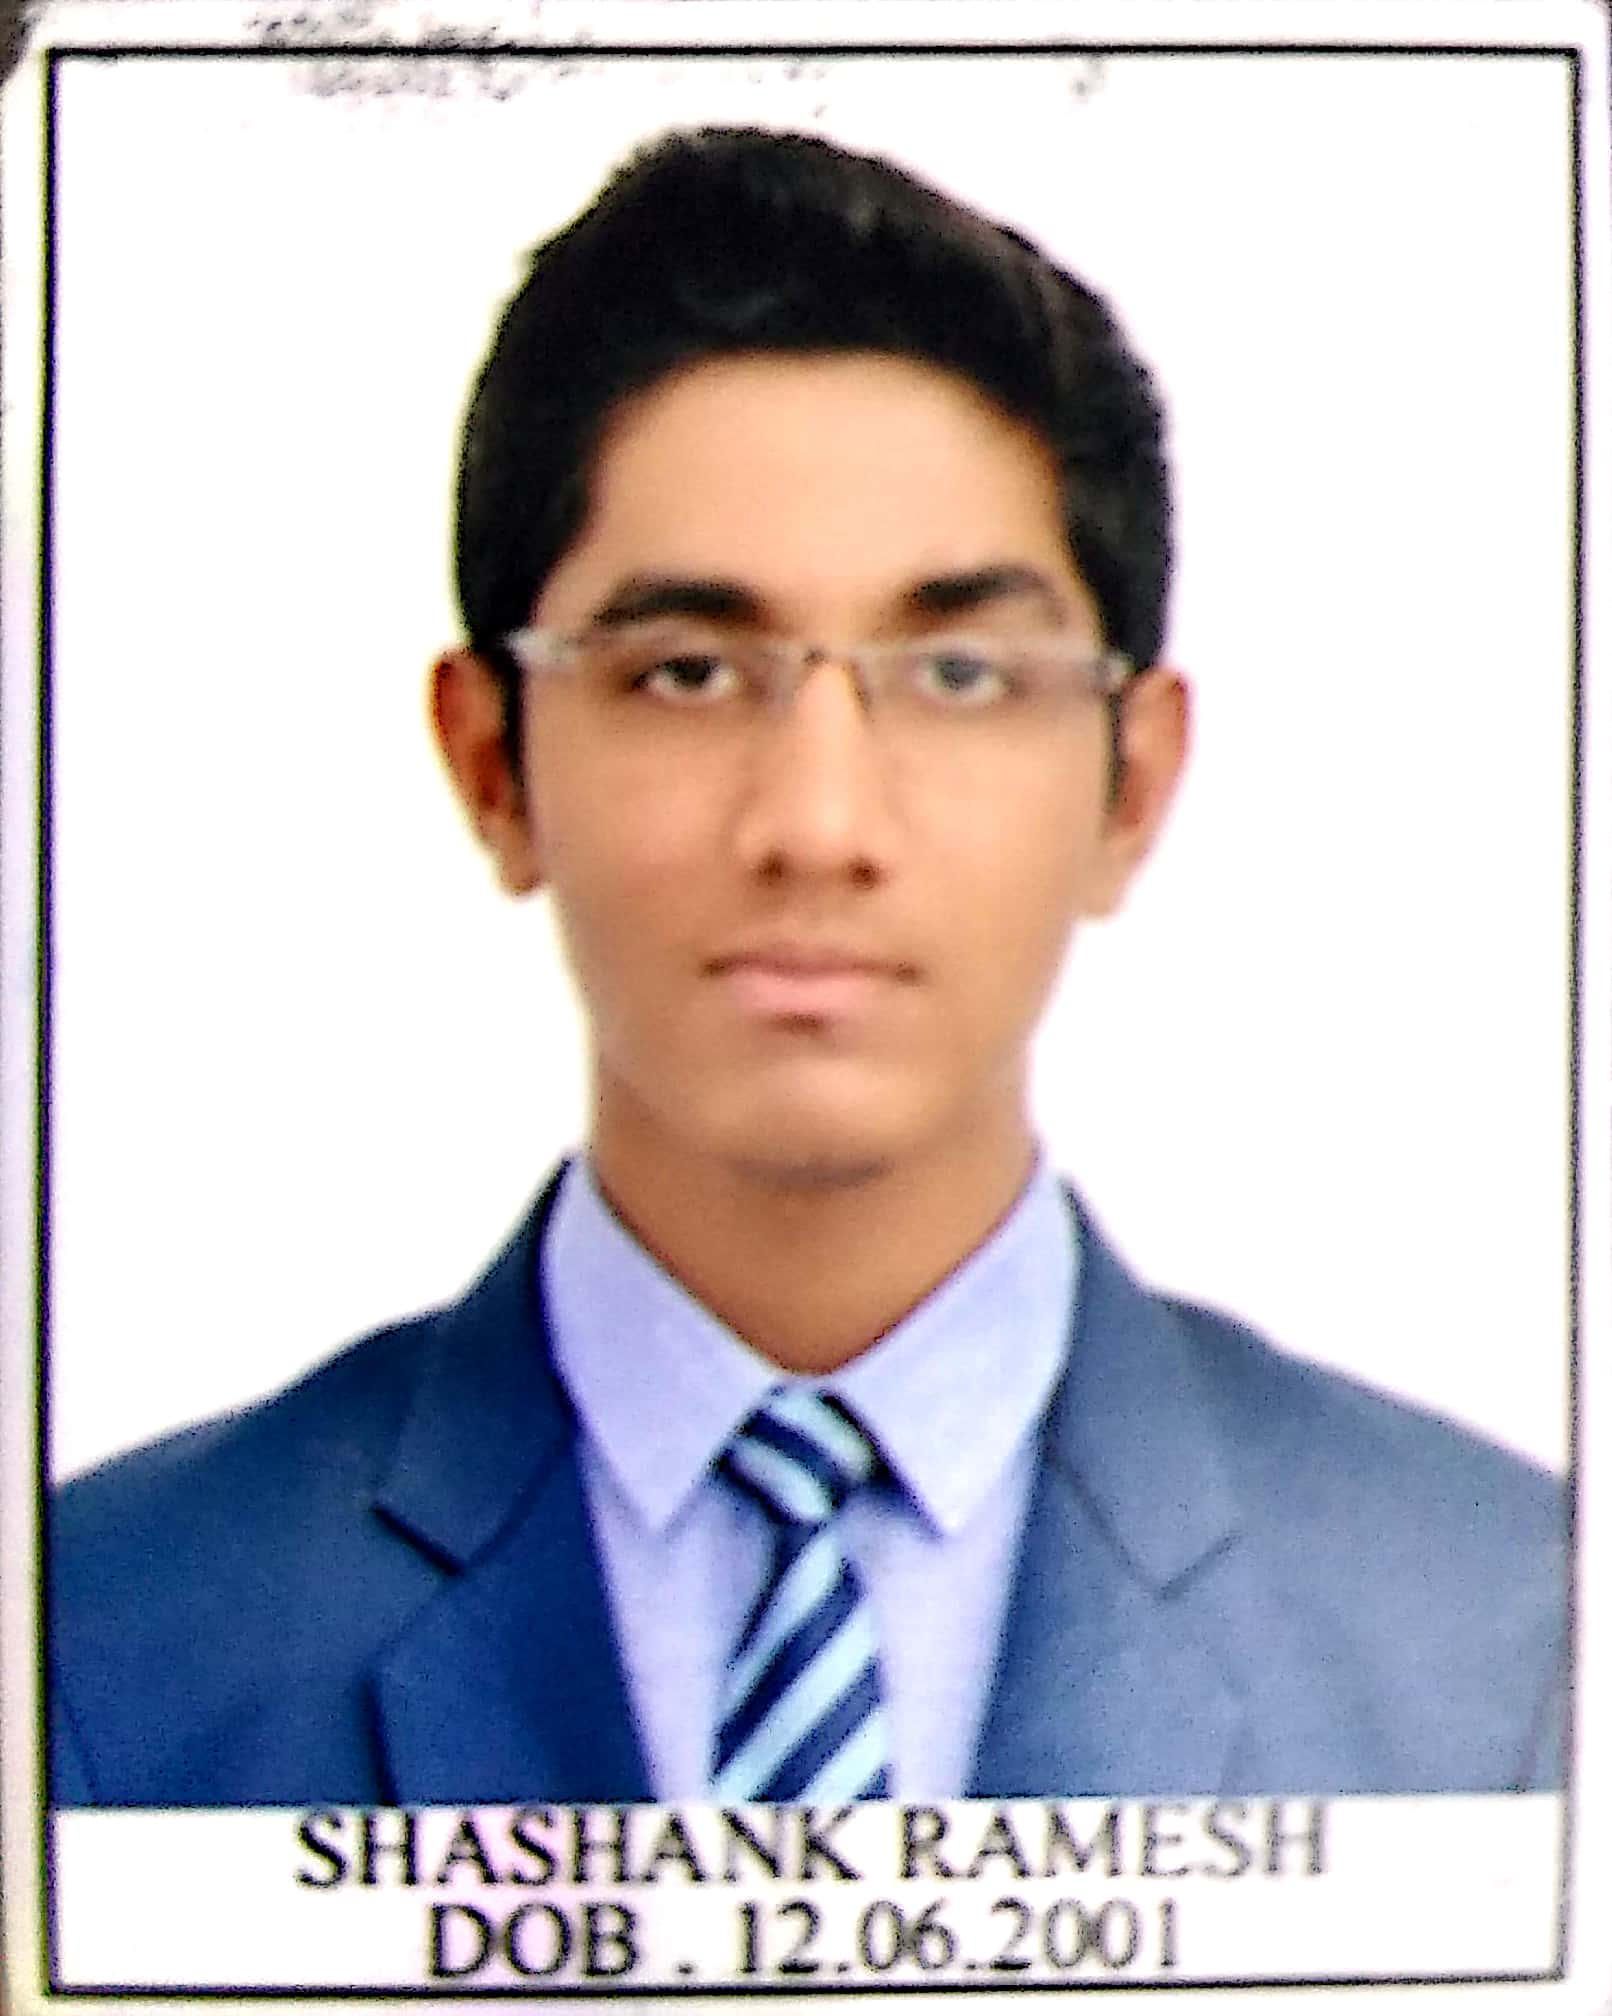
\includegraphics[width=1in,height=1.25in,clip,keepaspectratio]{shashank_photo}}]{Shashank Ramesh}
Shashank Ramesh is pursuing his B.Sc.(H) Physics at Kirori Mal College, University of Delhi. His academic interests lie in plasma physics and its applications in astrophysics.
\end{IEEEbiography} 
\vfill
\begin{IEEEbiography}[{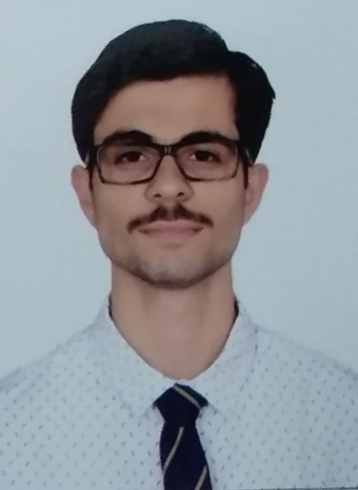
\includegraphics[width=1in,height=1.25in,clip,keepaspectratio]{chirag_photo}}]{Chirag Verma}
Chirag Verma is pursuing his B.Sc.(H) Physics at Kirori Mal College, University of Delhi. He has varied interests in theoretical and mathematical physics.
\end{IEEEbiography}
\vfill \vfill \vfill \vfill \vfill \vfill \vfill \vfill \vfill \vfill \vfill \vfill 
\vfill \vfill \vfill \vfill \vfill \vfill \vfill \vfill \vfill \vfill \vfill \vfill \vfill \vfill \vfill \vfill \vfill \vfill \vfill \vfill \vfill \vfill \vfill \vfill \vfill \vfill \vfill \vfill

 

\end{document}


